\documentclass[12pt,italian,a4paper,oneside,openright]{book}
\usepackage{url,amsfonts,epsfig}
\usepackage[italian]{babel}
\usepackage[utf8]{inputenc}
\usepackage[utf8]{inputenc}
\usepackage[format=hang,font=footnotesize]{caption}
\usepackage{vmargin}
\usepackage{amsmath}
\usepackage{indentfirst}
\usepackage{graphicx}
\usepackage{textcomp}
\usepackage{amssymb}
\usepackage{setspace}
\usepackage[linesnumbered,ruled,vlined]{algorithm2e}
\renewcommand{\thealgocf}{}
\usepackage[bottom]{footmisc}
\usepackage{xcolor}
\usepackage{listings}
\lstset{escapeinside={<@}{@>}}
\usepackage{minted}

\usepackage{etoolbox}
\apptocmd{\thebibliography}{\raggedright}{}{}

\usepackage[hyperindex]{hyperref} %per l'indice interattivo
\hypersetup{colorlinks=true, linkcolor=black} %per colorare i link


\begin{document}

{
    \thispagestyle{empty}
    
    \vskip 1cm \large \centerline{\textsc{Universit\`a degli Studi di
    Napoli ``Parthenope''}}
    
    \centerline {\textsc{Dipartimento di Scienze e Tecnologie}}
    
    \centerline {\small\textsc{Corso di laurea Triennale in Informatica}}
    \vskip 0.5cm

    \begin{center}
    
\includegraphics[scale=0.8]{img/logo.eps}
    \end{center}
    
    \vskip 0.5cm
    
    \large \centering {\textsc{Algoritmi e Strutture Dati e Laboratorio di Algoritmi e Strutture Dati}}
    
    \vskip 0.5cm
    
    \centerline {Relazione progetto traccia 2}
    
    \vskip 0.5cm

    \large
    \begin{minipage}[t]{7cm}
    \textsc{Docenti}
    
    Prof. Alessio Ferone\newline
    Prof. Francesco Camastra
    
    \end{minipage}
    \hfill
    \begin{minipage}[t]{6cm}
    \hfill \textsc{Candidato}
    
    \hfill Vittorio Fones 0124/1384
    \end{minipage}
    
    \vskip 1.0 cm \Large \centerline {Anno Accademico 2019-2020}
    \vfill \eject
} % fine frontespizio

\pagenumbering{Roman}
\baselineskip 1.5em

\markboth{Indice}{Indice}
\tableofcontents
\listoffigures
\newpage

\pagenumbering{arabic}
\part{}
\def\baselinestretch{1}
\chapter{Albero red-black di hash table}
\def\baselinestretch{1.66}
\thispagestyle{headings}

\def\baselinestretch{1}
\section{Descrizione problema}
\def\baselinestretch{1.66}
\thispagestyle{headings}

Il problema in analisi prevede di creare una struttura dati, in C++, che d'ora in avanti chiameremo
\textbf{red-black hash}, in grado di immagazzinare delle stringhe alfanumeriche. Tale struttura
\`e l'unione di un albero binario di ricerca bilanciato, \textbf{albero rosso-nero} o \textbf{albero
red-black}, e delle \textbf{hash table}: all'interno di ogni nodo di tale albero,
vi \`e presente una hash table, struttura dati che associa per ogni chiave un singolo valore, al cui
interno sono presenti delle stringhe. La traccia prevedeva di poter effettuare operazioni
\textbf{C.R.D.}\footnote{Create Retrieve Delete. Operazioni tipiche delle basi di dati, ma senza la
possibilit\`a di effettuare Updates.} su tuple nel formato: \verb|chiave1:chiave2:stringa| . 
La chiave 1 indicizza un nodo dell'albero red black, il quale puntando ad una hash
table utilizza la chiave 2 per associare la stringa.
Vi \`e quindi una relazione \verb|1:1| per i nodi dell'albero e l'hash table, e \verb|1:M| tra l'hash table
e le stringhe, dove \textbf{M} \`e la dimensione massima dell'hash table.

\def\baselinestretch{1}
\section{Descrizione strutture dati}
\def\baselinestretch{1.66}
\thispagestyle{headings}
\subsection{Alberi binari di ricerca}
\indent Gli \textbf{alberi binari di ricerca} sono delle strutture dati
 che immagazzinano dati in un albero avente in ogni nodo due 
 figli. Gli \textbf{ABR} (o in inglese BST) godono della seguente propriet\`a:
 $\forall \ x \in \ $BST$ :\ key(x.left) \leq key(x) < key(x.right)$. 
 Ovvero ogni nodo in un ABR ha come valore della chiave un valore
 maggiore del figlio sinistro ma minore di quello destro.
 \newline Ci\`o assicura operazioni in una complessit\`a 
 \textbf{logarimtica} data dalla profondit\`a dell'albero.
 Il problema sorge nel caso in cui avvengono cancellazioni
 sbagliate o inserimenti sbagliati che seppur mantengono
 la propriet\`a degli ABR, degradano tale albero in una lista concatenata
 compromettendo le operazioni di inserimento, cancellazione
 e ricerca ad avere complessit\`a lineare.

\subsection{Alberi Red-Black}
Gli alberi red black sono degli alberi binari di ricerca
\textbf{ autobilancianti }. Ogni volta che si inserisce un nuovo 
nodo, o lo 
si cancella si effettuano delle operazioni per bilanciare 
l'albero. Gli alberi rosso neri posseggono \textbf{5 propriet\`a} 
utili
ai metodi di supporto $insertFix()$ e $deleteFix()$ per garantire che le complessit\`a
peggiori abbiano al pi\`u come valore l'altezza dell'albero, ovvero $O(log_2n)$. 
I metodi di supporto all'inserimento e alla cancellazione fanno uso delle rotazioni di un nodo,
operazione che permette di compattare l'albero e garantire il corretto bilanciamento.
Di seguito verranno elencate tali propriet\`a:
\begin{itemize}
    \item ogni nodo \`e rosso o nero;
    \item la radice \`e nera;
    \item ogni foglia \`e nera;
    \item se un nodo \`e rosso, allora entrambi i suoi figli sono neri;
    \item per ogni nodo, tutti i cammini semplici che vanno dal nodo alle foglie sue discendenti
    contengono lo stesso numero di nodi neri.
\end{itemize}

\subsection{Hash Table ad indirizzamento aperto}
Le \textbf{Hash Table}, o hash map, sono delle strutture dati che permettono di associare ad una
chiave un singolo valore. Precisamente ad ogni chiave va applicata una funzione detta funzione
di hashing che calcoler\`a un indice. Pu\`o capitare per\`o che una funzione hash applicata su chiavi diverse 
indicizzi celle simili dell'hashtable, per tanto bisogna gestire queste \textit{collisioni}.
La tavola hash realizzata \`e del tipo a \textbf{indirizzamento aperto}, ovvero non facendo
uso dei puntatori si \textit{ispeziona} l'hashtable fino a incontrare una posizione libera,
se presente. Il metodo di ispezione scelto \`e quello del \textbf{doppio hashing}: rispetto
ad altre ispezioni, quella del doppio hashing trova una posizione in modo pi\`u veloce.
Nei capitoli successivi vedremo nel dettaglio il funzionamento.
\newpage
\def\baselinestretch{1}
\section{Formato di input e di output}
\def\baselinestretch{1.66}
\thispagestyle{headings}

\subsection{Input}
I dati in input del problema sono:
\begin{itemize}
    \item V: numero intero di Vertici del grafo
    \item E: numero intero di Archi del grafo
    \item W: numero intero di Wormholes presenti nel grafo
    \item Tuple rappresentante archi: NodoA, NodoB, Peso
    \footnote{ndr: NodoA e NodoB sono le chiavi intere dei vertici
    e Peso \`e un intero usato per rappresentare il peso di tale
    arco.}
\end{itemize}
Tali dati sono immagazzinati in un file di testo non binario
contenente nel primo rigo i primi tre dati elencati, mentre nei
successivi sono presenti le \textbf{tuple}.
Per rappresentare i wormhole il programma prende gli \textbf{
ultimi W NodiB} contenuti nel file e li va a salvare in un
vettore di vertici.

\subsection{Output}
Il programma sviluppato restituisce in output i nodi che collegano
la coppia \textbf{sorgente - destinazione} nel minor "tempo" possibile 
e il relativo costo di tale cammino minino, \textbf{se esiste}:
pu\`o capitare, come vedremo nel paragrafo \textit{"Test effettuati" par. \ref{notconn}},
che il grafo non sia connesso e che il nodo destinazione sia raggiungibile 
solo attraverso i vertici di tipo wormhole.
Inoltre il programma restituisce, il cammino minimo (vertici da attraversare
e costo totale) facendo uso dei nodi speciali wormhole. L'output secondario
pu\`o mancare nel caso in cui non si incontrino wormhole, oppure il wormhole di partenza \`e uguale a quello di destinazione.\newpage
\def\baselinestretch{1}
\section{Descrizione algoritmo}
\def\baselinestretch{1.66}
\thispagestyle{headings}
\subsection{Pseudo codice}

L'insertimento nella struttura dati creata va effettuare prima una ricerca
del nodo di chiave $key1$. Se dovesse riscontrare un esito negativo si procede
alla allocazione di un hashtable e un nuovo nodo. In caso contrario si procede alla ricerca
di una cella della tavola di hash con la $key2$, se anche questa ricerca restituisce un esito
negativo allora si procede con l'inserimento.

\BlankLine
\IncMargin{1.5em}
\begin{algorithm}[H]
\setstretch{1.1}
\caption{Insert}
\SetKwData{Left}{left}\SetKwData{This}{this}\SetKwData{Up}{up}
\SetKwFunction{Union}{Union}\SetKwFunction{FindCompress}{FindCompress}
\SetKwInOut{Input}{input}\SetKwInOut{Result}{result}
\SetKwIF{If}{ElseIf}{Else}{if}{:}{elif}{else:}{}
\Input{ key1, key2, string }
\Result{boolean}
\emph{$node$ = Search in Red Black with $key1$}\;
\If{$\nexists \ node$} {
    \emph{new Hashtable()}\;
    \emph{new Node()}\;
    \emph{Hashtable.insert(key2, string)}\;
    \emph{Node.insert(key1, Hashtable)}\;
    return \emph{true}\;
}
\Else{\If{$\nexists \ node.Hashtable.search(key2)$} {
        \emph{node.Hashtable.insert(key2, d)}\;
        return \emph{true}\; }}
return \emph{false}\;
\end{algorithm}\newpage
\indent La ricerca controlla la correttezza delle chiavi e della stringa inserita nella tupla:
in caso di riscontro positivo la function ritorner\`a il nodo dell'albero.
\BlankLine
\IncMargin{1.5em}
\begin{algorithm}[H]
\setstretch{1.1}
\caption{Search (retrieve) }
\SetKwData{Left}{left}\SetKwData{This}{this}\SetKwData{Up}{up}
\SetKwFunction{Union}{Union}\SetKwFunction{FindCompress}{FindCompress}
\SetKwInOut{Input}{input}\SetKwInOut{Result}{result}
\SetKwIF{If}{ElseIf}{Else}{if}{:}{elif}{else:}{}
\Input{ key1, key2, string }
\Result{node if found $or$ NIL if not found}
\emph{$node$ = Search in Red Black with $key1$}\;
\If{$\exists \ node$} {
    \emph{$data$ = node.Hashtable.search(key2)}\;
    \If{string = data } {
        return \emph{node}\;
    }
}
return \emph{NIL}\;
\end{algorithm}\newpage

\indent La cancellazione di una tupla effettua una operazione di ricerca nella struttura dati.
Se la ricerca ha risconto positivo allora si procede con i due casi della rimozione:
se la chiave secondaria indicizza una hashtable in cui vi \`e presente un solo elemento, allora
si canceller\`a l'intero nodo red black, altrimenti si procede alla normale rimozione dalla hashtable.
\BlankLine
\IncMargin{1.5em}
\begin{algorithm}[H]
\setstretch{1.1}
\caption{Remove (delete)}
\SetKwData{Left}{left}\SetKwData{This}{this}\SetKwData{Up}{up}
\SetKwFunction{Union}{Union}\SetKwFunction{FindCompress}{FindCompress}
\SetKwInOut{Input}{input}\SetKwInOut{Result}{result}
\SetKwIF{If}{ElseIf}{Else}{if}{:}{elif}{else:}{}
\Input{ key1, key2, string }
\Result{true if deleted $or$ false if not}
\emph{node = Search in Red Black Hash}\;
\If{$node \neq NIL$} {
    \eIf{node.Hashtable.capacity = 1} {
    \emph{delete node}\;}
    {node.Hashtable.remove(key2)\;}
    return \emph{true}\;}
return \emph{false}\;
\end{algorithm}\newpage

\subsection{Diagrammi delle classe e dettagli architetturali}
\subsubsection{Nodi Binari}
\indent I nodi facenti parti degli alberi
binari sono nodi che derivano da una classe astratta che a sua
volta estende un nodo generico.\newline
\indent Per permettere agli alberi binari di usare come parametro
templato un generico nodo, si \`e sfruttato un particolare
pattern strutturale chiamato \textbf{CRTP} \textit{(Curiously recurring 
template pattern)}: una classe (e.g. ConcreteBinaryNode) eredita
da una classe base template (e.g. AbstractBinaryNode), usando
come parametro di specializzazione se stessa. Il nodo concreto
RedBlack in pi\`u implementa la classe color. Si \`e scelta tale tecnica che non porta
miglioramenti sostanziali al codice se non quella di nascondere
dettagli implementativi e un' indipendenza dalla rappresentazione in memoria del colore.
\begin{center}
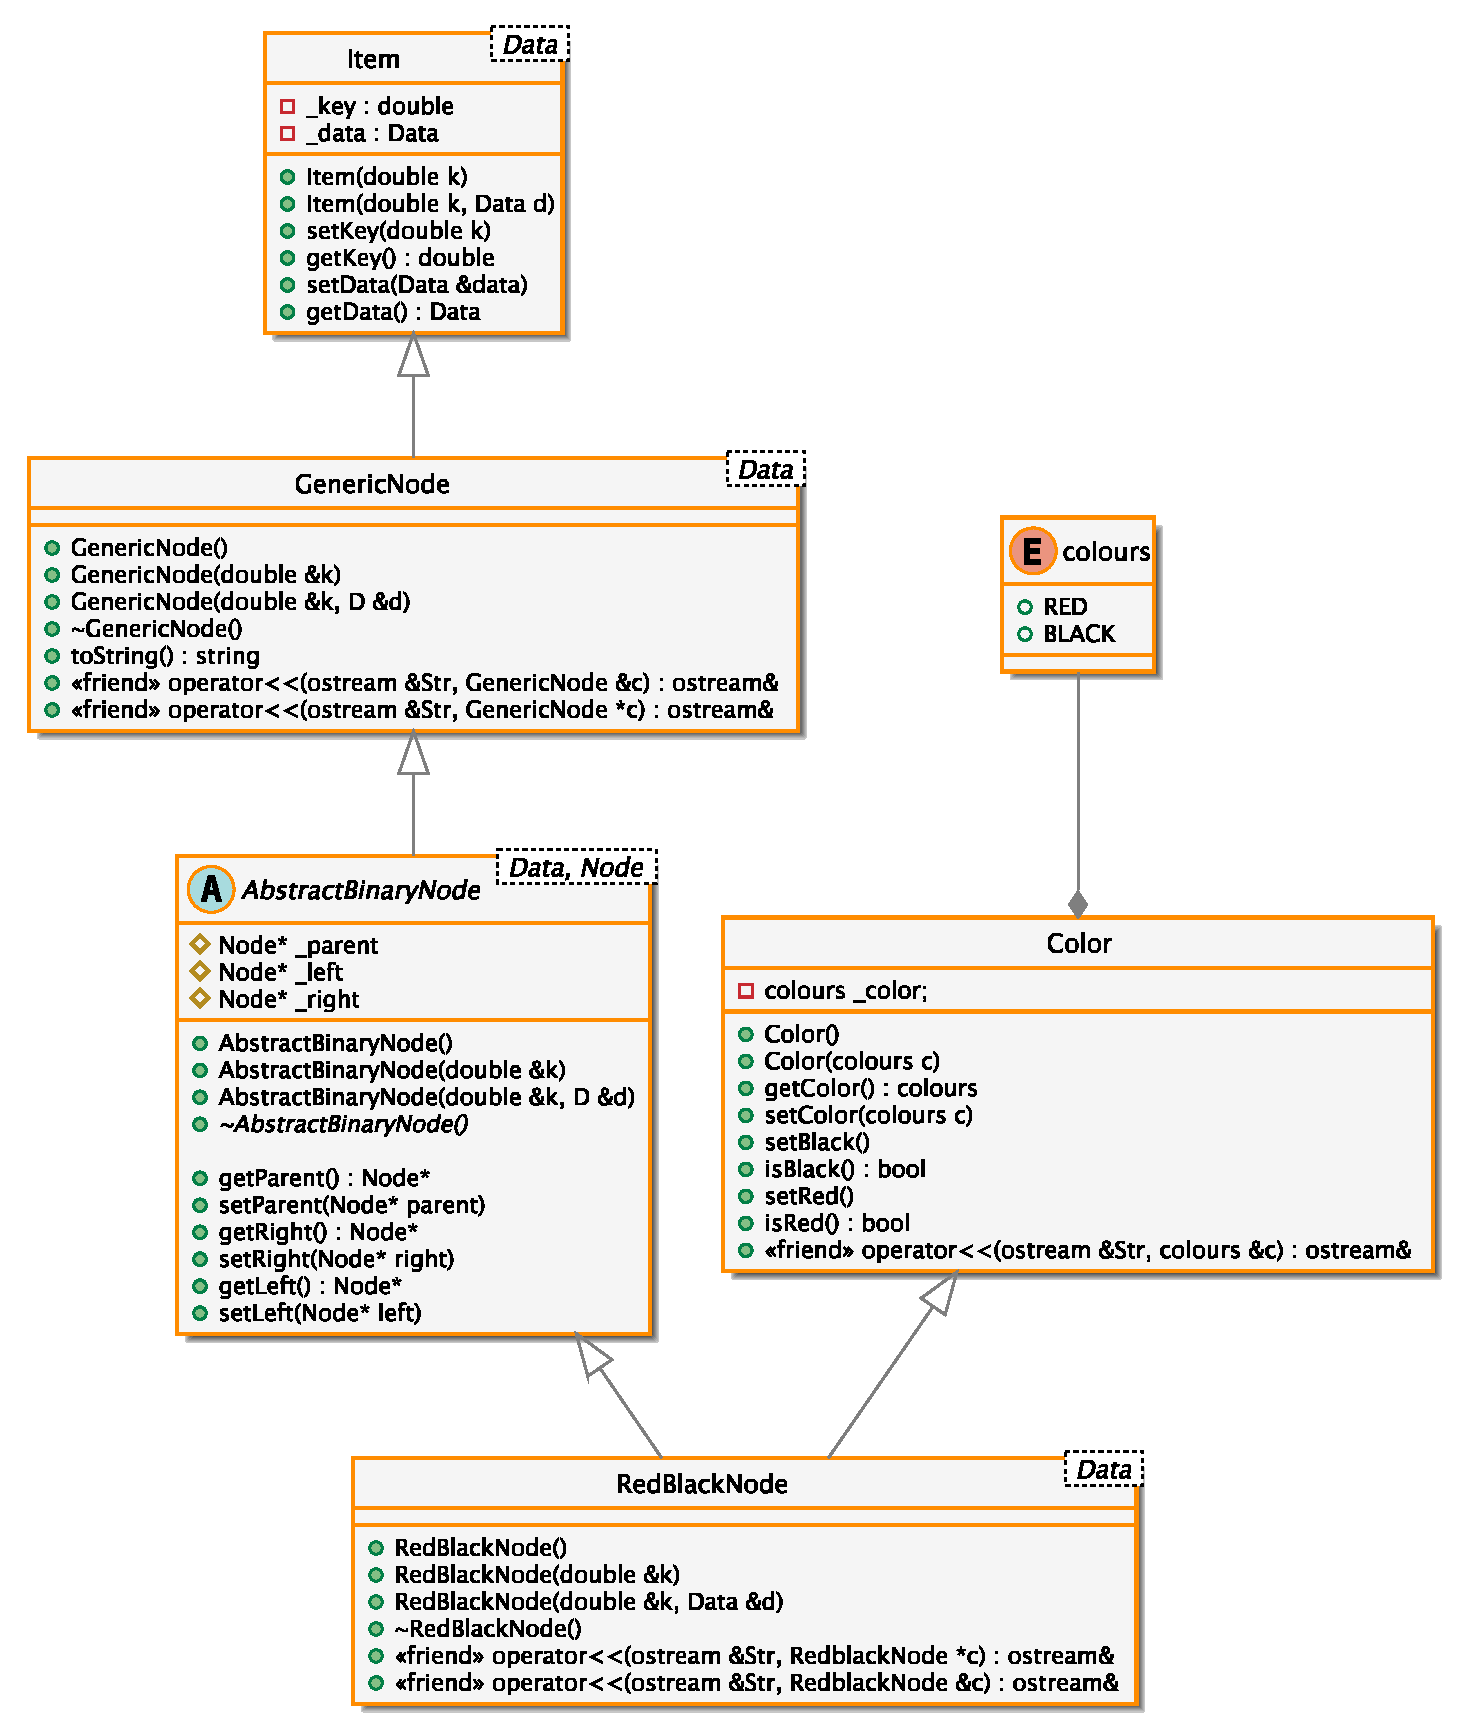
\includegraphics[scale=0.6]{tesina_tex/rbhash/2img/nodes.eps}
\captionof{figure}{Nodi degli alberi}
\end{center}
\subsubsection{Alberi}
Un albero Rosso Nero \`e un albero binario di ricerca auto
bilanciante, per tanto si \`e scelto di estendere la classe
BinarySearchTree ed aggiungere i metodi di supporto al bilanciamento. Inoltre due metodi virtuali (insert e delete), sono
stati ridefiniti nell'implementazione del Red Black.
\textit{insertNode} richiama tramite lo scope della classe
BinarySearchTree la insert e successivamente applica il
\textbf{fix} tipico dei red black.
\begin{center}
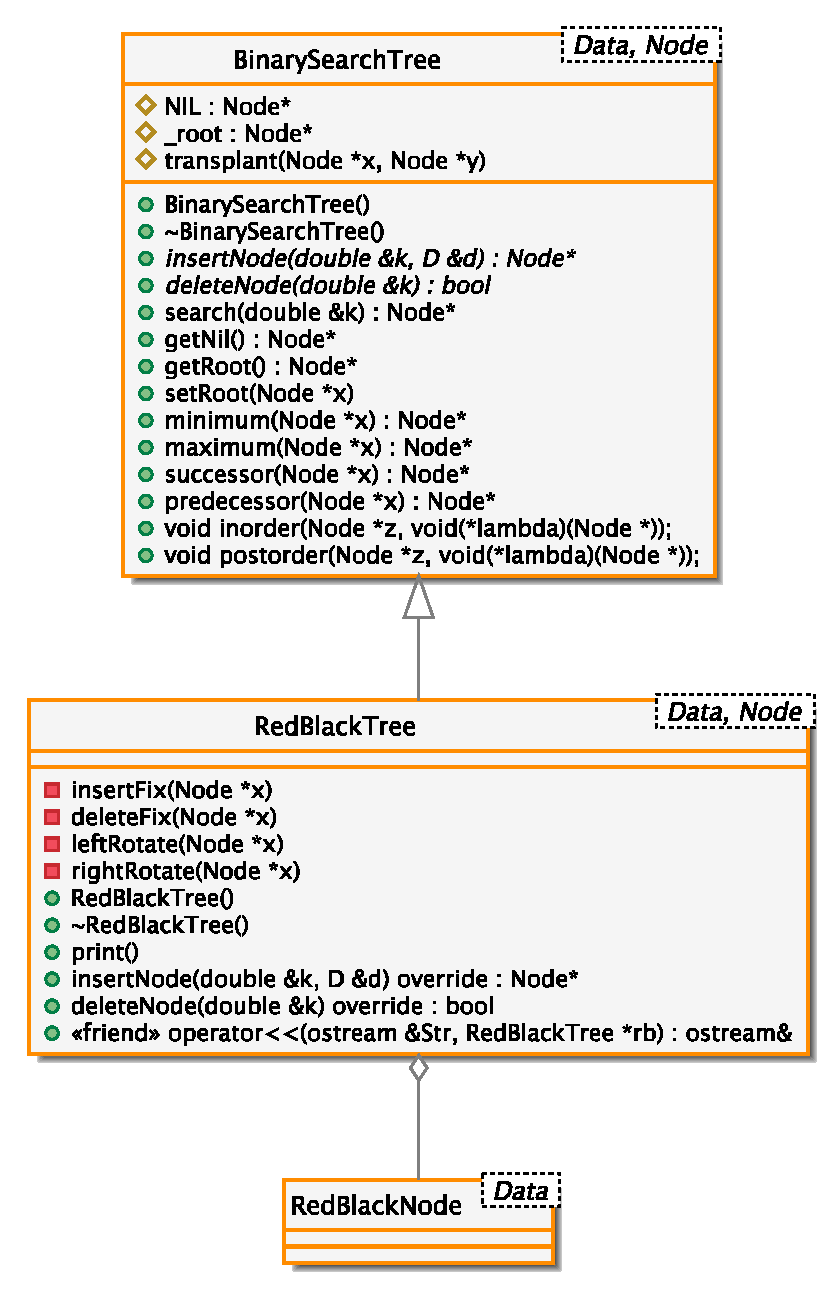
\includegraphics[scale=0.6]{tesina_tex/rbhash/2img/trees.eps}
\captionof{figure}{Alberi}
\end{center}
\subsection{Hash Table}
Onde evitare di dover riscrivere codice si \`e scelto di sfruttare
il nodo generico anche per l'\textbf{HashTable}. A tal proposito
si \`e sviluppato una tabella hash ad \textbf{indirizzamento aperto} che
prende in input come paramentro templato, il dato da conservare e 
la funzione di hash sotto forma di classe.
Per risolvere le collisioni si \`e scelto di usare due funzioni hash:
\texttt{k} \`e un valore double che indica
la chiave, $\texttt{i}$ \`e l'iteratore che al massimo 
$\texttt{m}$ volte \footnote{m \`e il size dell'hashtable}  
applicher\`a la funzione di hash. La prima restituisce un indice con valore compreso
tra $[0, m]$, mentre la seconda funzione di hash un valore compreso tra $[1, m-1]$. 
Verr\`a usata la prima funzione di hash e in caso di collisione
si riapplicher\`a
$h(i, m) = (h_1(k) + i * h_2(k)) \ mod \ m$. Sebbene con un costo 
computazionale pi\`u alto, il doppio hashing risolve le collisioni
pi\`u in fretta rispetto allispezione lineare o quadratica.\newline \indent 
La funzione $search()$ nella class \textbf{HashTable} usa due
diversi parametri di input per restituire valori diversi. Con la 
ricerca per valore si restituise, se disponibile un indice che 
usato nella seconda funzione di ricerca restituisce il dato.

\begin{center}
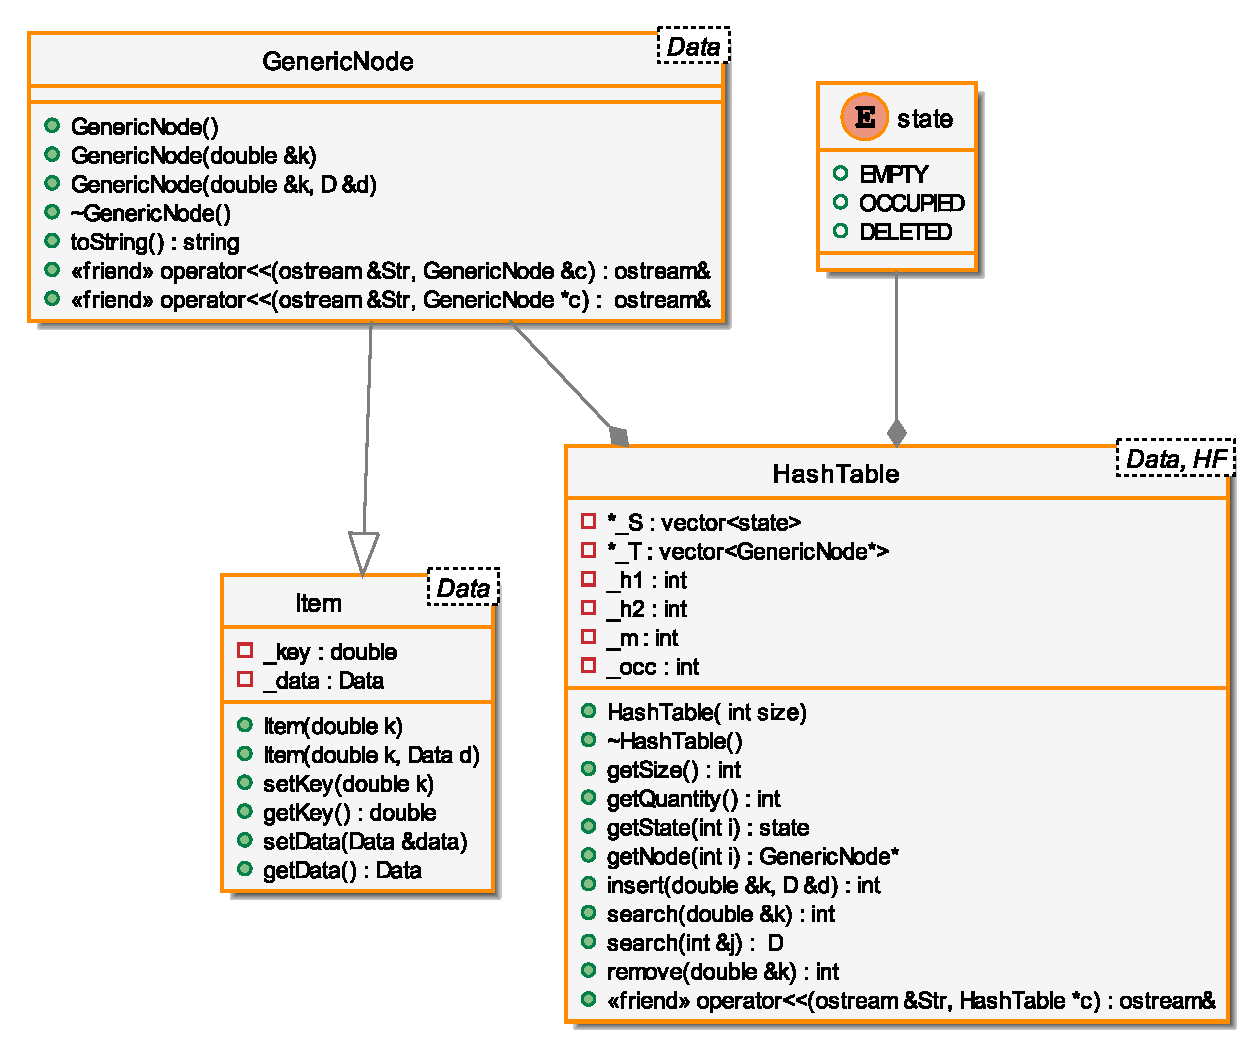
\includegraphics[scale=0.6]{tesina_tex/rbhash/2img/hash.eps}
\captionof{figure}{Hash Table}
\end{center}\newpage
\def\baselinestretch{1}
\section{Studio complessit\`a}
\def\baselinestretch{1.66}
\thispagestyle{headings}
La complessit\`a di tempo data dall'algoritmo galactic dijkstra \`e influenzata
dalle \textbf{due esecuzioni} (al pi\`u) del classico algoritmo di Dijkstra. Il calcolo
dei percorsi impiega $O(3E)$ poich\'e per raggiungere un nodo fino alla sorgente vuol dire
ripercorrere l'albero attraversando ogni arco nel caso peggiore, quindi mettendoci un tempo lineare.
Per cui si considerano le due applicazioni di Dijkstra che impiegano $O(2(V+E) 2log_2 V)$ che diventa
$O(2E2log_2 V)$ se ogni vertice \`e raggiungibile dalla sorgente, ma poich\`e è possibile portare
le costanti moltiplicative fuori diremo che la complessit\`a finale sar\`a $\mathbf{O(Elog_2V)}$.
L'algoritmo di Dijkstra impiega tale complessit\`a poich\'e influenzato dalle operazioni
$extractMin()$ e $decreaseKey()$ impiegate $|E|$ volte dalla coda di min priorit\`a basata
su min heap.
Si poteva pensare di usare un Heap di Fibonacci poich\'e si \`e notato che l'algoritmo
effettua pi\`u operazioni di $decreaseKey()$ che di $extractMin()$, e nella struttura dati
citata tale operazioni hanno rispettivamente costo computazionale $O(1)$ e $O(log_2V)$. Ci\`o
avrebbe comportato un miglioramento nel caso in cui ci fossero stati molti archi, avendo un costo
asintotico pari a $O(Vlog_2V +E)$.\newpage
\def\baselinestretch{1}
\section{Test e risultati}
\def\baselinestretch{1.66}
\thispagestyle{headings}

\subsection{Test effettuati}\label{notconn}
I risultati estratti da una shell dopo aver eseguito il programma prevedono vari grafi. Per ognuno
di essi vi sar\`a presente il grafico relativo.

\begin{center}
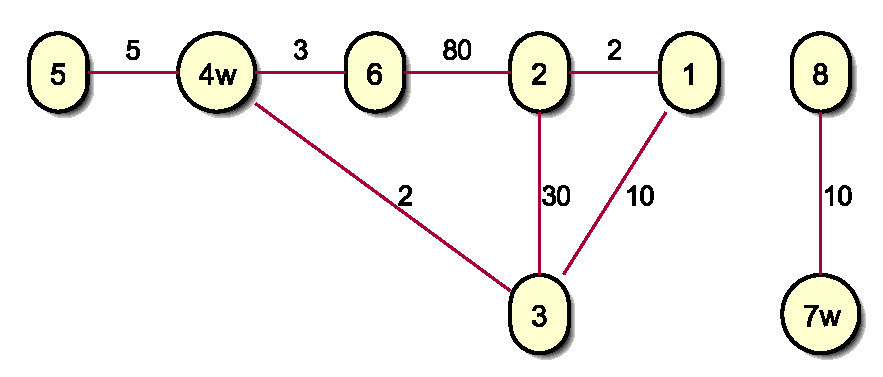
\includegraphics[scale=0.7]{tesina_tex/spacegraph/2img/notconn.eps}
\captionof{figure}{Grafo non connesso.}
\end{center}

\begin{minted}{bash}
Filling a graph with 8 nodes, 8 edges, 2 wormholes
STARTING READING FILE: 6
STARTING READING 2ndhalf: 2

Looking for a path from 1 to 8

Travel without wormholes: there are no paths that connect 1 with 8
        (disconnected graph)

Using wormholes -> [4, 7]: 1-3-4^7-8 in 23 unit time
\end{minted}

\newpage

\begin{center}
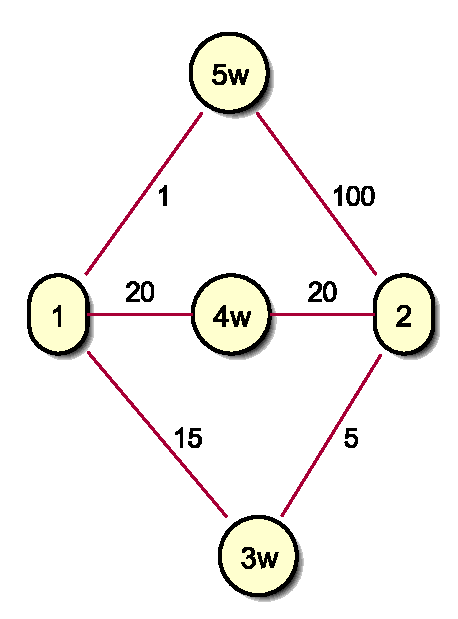
\includegraphics[scale=0.7]{tesina_tex/spacegraph/2img/diamond.eps}
\captionof{figure}{Grafo a diamante.}
\end{center}

\begin{minted}{bash}
Filling a graph with 5 nodes, 6 edges, 3 wormholes
STARTING READING FILE: 3
STARTING READING 2ndhalf: 3

Looking for a path from 1 to 2

Travel without wormholes: 1-3-2 in 20 time unit

Using wormholes -> [5, 3]: 1-5^3-2 in 7 unit time
\end{minted}



\newpage Nel grafo seguente il percorso con wormhole non \`e mostrato in quanto il wormhole
usato dalla sorgente e dalla destizione \`e lo stesso, infatti il nodo $11$ \`e presente
in entrambi i cammini minimi.
\begin{center}
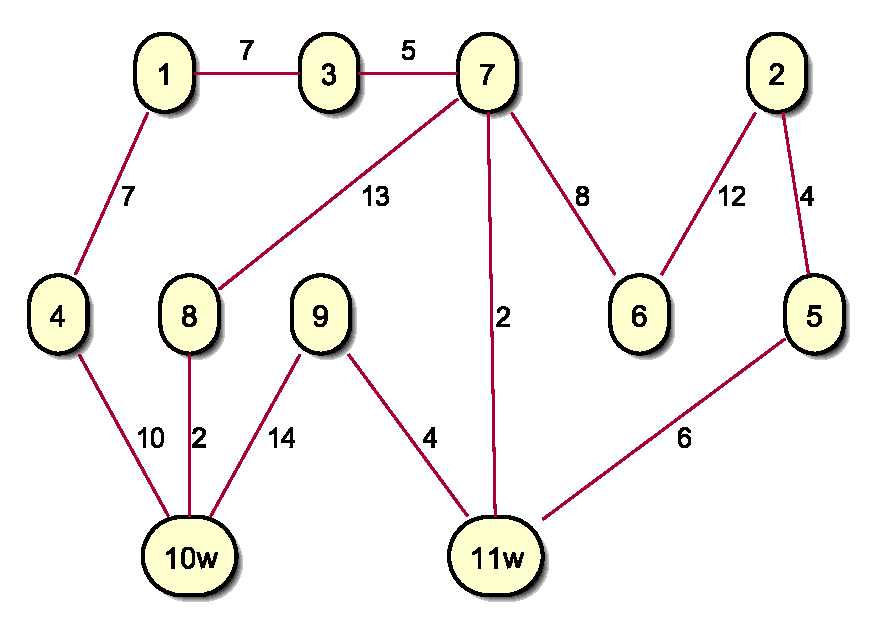
\includegraphics[scale=0.7]{tesina_tex/spacegraph/2img/traccia.eps}
\captionof{figure}{Grafo d'esempio.}
\end{center}

\begin{minted}{bash}
Filling a graph with 11 nodes, 13 edges, 2 wormholes
STARTING READING FILE: 11
STARTING READING 2ndhalf: 2

Looking for a path from 1 to 2

Travel without wormholes: 1-3-7-11-5-2 in 24 time unit

No fast travel with wormhole.
\end{minted}




\newpage Per puro stress testing del programma, si \`e utilizzato un file contentente
317080 nodi, 1049866 archi e 10 wormholes, ovviamente previo
commento nell'implementazione
del parser circa i controlli sull'input. Successimante si usa lo stesso file ma senza
wormhole in modo da non far applicare una seconda volta dijkstra.
Il risultato mostrato di seguito contiene l'esecuzione calcolandone i tempi tramite
l'applicativo \emph{time} presente nei sistemi operativi \emph{*NIX}

\begin{minted}[breaklines=true]{bash}
Filling a graph with 317080 nodes, 1049866 edges, 10 wormholes
STARTING READING FILE: 1049856
STARTING READING 2ndhalf: 10

Looking for a path from 316972 to 317029

Travel without wormholes:
316972-264079-298841-63506-59115-5530-26742-65338
-191800-287822-125483-121155-107180-308349-317029
in 104 time unit

Using wormholes -> [316972, 317029]: 316972^317029 in 1 unit time


real    1m42.700s
user    1m42.313s
sys     0m0.188s
\end{minted}
\newpage
Da notare come il file senza wormhole ci impiega circa la \textbf{met\`a}.

\begin{minted}[breaklines=true]{bash}
Filling a graph with 317080 nodes, 1049866 edges, 0 wormholes
STARTING READING FILE: 1049866
STARTING READING 2ndhalf: 0

Looking for a path from 316972 to 317029

Travel without wormholes:
316972-264079-298841-63506-59115-5530-26742-65338
-191800-287822-125483-121155-107180-308349-317029
in 104 time unit

No wormhole from Source to Destination.

real    0m56.303s
user    0m56.047s
sys     0m0.094s

\end{minted}

\newpage
\def\baselinestretch{1}
\section{Codice sorgente}
\def\baselinestretch{1.66}
\thispagestyle{headings}

\inputminted
[fontsize=\small,baselinestretch=1,
frame=lines,
framesep=10pt,
linenos=true,tabsize=2,
breaklines=true]{c++}{tesina_tex/source/graph/heap.hpp}
\inputminted
[fontsize=\small,baselinestretch=1,
frame=lines,
framesep=10pt,
linenos=true,tabsize=2,
breaklines=true]{c++}{tesina_tex/source/graph/heap.cpp}

\newpage
\inputminted
[fontsize=\small,baselinestretch=1,
frame=lines,
framesep=10pt,
linenos=true,tabsize=2,
breaklines=true]{c++}{tesina_tex/source/graph/minHeap.hpp}
\inputminted
[fontsize=\small,baselinestretch=1,
frame=lines,
framesep=10pt,
linenos=true,tabsize=2,
breaklines=true]{c++}{tesina_tex/source/graph/minHeap.cpp}
\newpage
\inputminted
[fontsize=\small,baselinestretch=1,
frame=lines,
framesep=10pt,
linenos=true,tabsize=2,
breaklines=true]{c++}{tesina_tex/source/graph/minPriorityQueue.hpp}
\inputminted
[fontsize=\small,baselinestretch=1,
frame=lines,
framesep=10pt,
linenos=true,tabsize=2,
breaklines=true]{c++}{tesina_tex/source/graph/minPriorityQueue.cpp}
\newpage


\inputminted
[fontsize=\small,baselinestretch=1,
frame=lines,
framesep=10pt,
linenos=true,tabsize=2,
breaklines=true]{c++}{tesina_tex/source/graph/galacticgraph.hpp}
\inputminted
[fontsize=\small,baselinestretch=1,
frame=lines,
framesep=10pt,
linenos=true,tabsize=2,
breaklines=true]{c++}{tesina_tex/source/graph/galacticgraph.cpp}
\newpage

\inputminted
[fontsize=\small,baselinestretch=1,
frame=lines,
framesep=10pt,
linenos=true,tabsize=2,
breaklines=true]{c++}{tesina_tex/source/graph/loader.hpp}
\inputminted
[fontsize=\small,baselinestretch=1,
frame=lines,
framesep=10pt,
linenos=true,tabsize=2,
breaklines=true]{c++}{tesina_tex/source/graph/loader.cpp}
\newpage

\inputminted
[fontsize=\small,baselinestretch=1,
frame=lines,
framesep=10pt,
linenos=true,tabsize=2,
breaklines=true]{c++}{tesina_tex/source/graph/debug.hpp}
\inputminted
[fontsize=\small,baselinestretch=1,
frame=lines,
framesep=10pt,
linenos=true,tabsize=2,
breaklines=true]{c++}{tesina_tex/source/graph/item.hpp}
\newpage

\inputminted
[fontsize=\small,baselinestretch=1,
frame=lines,
framesep=10pt,
linenos=true,tabsize=2,
breaklines=true]{c++}{tesina_tex/source/graph/vertex.hpp}
\inputminted
[fontsize=\small,baselinestretch=1,
frame=lines,
framesep=10pt,
linenos=true,tabsize=2,
breaklines=true]{c++}{tesina_tex/source/graph/vertex.cpp}
\newpage

\inputminted
[fontsize=\small,baselinestretch=1,
frame=lines,
framesep=10pt,
linenos=true,tabsize=2,
breaklines=true]{c++}{tesina_tex/source/graph/graph.hpp}
\inputminted
[fontsize=\small,baselinestretch=1,
frame=lines,
framesep=10pt,
linenos=true,tabsize=2,
breaklines=true]{c++}{tesina_tex/source/graph/graph.cpp}
\newpage\newpage

\part{}
\def\baselinestretch{1}
\chapter{Albero red-black di hash table}
\def\baselinestretch{1.66}
\thispagestyle{headings}

\def\baselinestretch{1}
\section{Descrizione problema}
\def\baselinestretch{1.66}
\thispagestyle{headings}

Il problema in analisi prevede di creare una struttura dati, in C++, che d'ora in avanti chiameremo
\textbf{red-black hash}, in grado di immagazzinare delle stringhe alfanumeriche. Tale struttura
\`e l'unione di un albero binario di ricerca bilanciato, \textbf{albero rosso-nero} o \textbf{albero
red-black}, e delle \textbf{hash table}: all'interno di ogni nodo di tale albero,
vi \`e presente una hash table, struttura dati che associa per ogni chiave un singolo valore, al cui
interno sono presenti delle stringhe. La traccia prevedeva di poter effettuare operazioni
\textbf{C.R.D.}\footnote{Create Retrieve Delete. Operazioni tipiche delle basi di dati, ma senza la
possibilit\`a di effettuare Updates.} su tuple nel formato: \verb|chiave1:chiave2:stringa| . 
La chiave 1 indicizza un nodo dell'albero red black, il quale puntando ad una hash
table utilizza la chiave 2 per associare la stringa.
Vi \`e quindi una relazione \verb|1:1| per i nodi dell'albero e l'hash table, e \verb|1:M| tra l'hash table
e le stringhe, dove \textbf{M} \`e la dimensione massima dell'hash table.

\def\baselinestretch{1}
\section{Descrizione strutture dati}
\def\baselinestretch{1.66}
\thispagestyle{headings}
\subsection{Alberi binari di ricerca}
\indent Gli \textbf{alberi binari di ricerca} sono delle strutture dati
 che immagazzinano dati in un albero avente in ogni nodo due 
 figli. Gli \textbf{ABR} (o in inglese BST) godono della seguente propriet\`a:
 $\forall \ x \in \ $BST$ :\ key(x.left) \leq key(x) < key(x.right)$. 
 Ovvero ogni nodo in un ABR ha come valore della chiave un valore
 maggiore del figlio sinistro ma minore di quello destro.
 \newline Ci\`o assicura operazioni in una complessit\`a 
 \textbf{logarimtica} data dalla profondit\`a dell'albero.
 Il problema sorge nel caso in cui avvengono cancellazioni
 sbagliate o inserimenti sbagliati che seppur mantengono
 la propriet\`a degli ABR, degradano tale albero in una lista concatenata
 compromettendo le operazioni di inserimento, cancellazione
 e ricerca ad avere complessit\`a lineare.

\subsection{Alberi Red-Black}
Gli alberi red black sono degli alberi binari di ricerca
\textbf{ autobilancianti }. Ogni volta che si inserisce un nuovo 
nodo, o lo 
si cancella si effettuano delle operazioni per bilanciare 
l'albero. Gli alberi rosso neri posseggono \textbf{5 propriet\`a} 
utili
ai metodi di supporto $insertFix()$ e $deleteFix()$ per garantire che le complessit\`a
peggiori abbiano al pi\`u come valore l'altezza dell'albero, ovvero $O(log_2n)$. 
I metodi di supporto all'inserimento e alla cancellazione fanno uso delle rotazioni di un nodo,
operazione che permette di compattare l'albero e garantire il corretto bilanciamento.
Di seguito verranno elencate tali propriet\`a:
\begin{itemize}
    \item ogni nodo \`e rosso o nero;
    \item la radice \`e nera;
    \item ogni foglia \`e nera;
    \item se un nodo \`e rosso, allora entrambi i suoi figli sono neri;
    \item per ogni nodo, tutti i cammini semplici che vanno dal nodo alle foglie sue discendenti
    contengono lo stesso numero di nodi neri.
\end{itemize}

\subsection{Hash Table ad indirizzamento aperto}
Le \textbf{Hash Table}, o hash map, sono delle strutture dati che permettono di associare ad una
chiave un singolo valore. Precisamente ad ogni chiave va applicata una funzione detta funzione
di hashing che calcoler\`a un indice. Pu\`o capitare per\`o che una funzione hash applicata su chiavi diverse 
indicizzi celle simili dell'hashtable, per tanto bisogna gestire queste \textit{collisioni}.
La tavola hash realizzata \`e del tipo a \textbf{indirizzamento aperto}, ovvero non facendo
uso dei puntatori si \textit{ispeziona} l'hashtable fino a incontrare una posizione libera,
se presente. Il metodo di ispezione scelto \`e quello del \textbf{doppio hashing}: rispetto
ad altre ispezioni, quella del doppio hashing trova una posizione in modo pi\`u veloce.
Nei capitoli successivi vedremo nel dettaglio il funzionamento.
\newpage
\def\baselinestretch{1}
\section{Formato di input e di output}
\def\baselinestretch{1.66}
\thispagestyle{headings}

\subsection{Input}
I dati in input del problema sono:
\begin{itemize}
    \item V: numero intero di Vertici del grafo
    \item E: numero intero di Archi del grafo
    \item W: numero intero di Wormholes presenti nel grafo
    \item Tuple rappresentante archi: NodoA, NodoB, Peso
    \footnote{ndr: NodoA e NodoB sono le chiavi intere dei vertici
    e Peso \`e un intero usato per rappresentare il peso di tale
    arco.}
\end{itemize}
Tali dati sono immagazzinati in un file di testo non binario
contenente nel primo rigo i primi tre dati elencati, mentre nei
successivi sono presenti le \textbf{tuple}.
Per rappresentare i wormhole il programma prende gli \textbf{
ultimi W NodiB} contenuti nel file e li va a salvare in un
vettore di vertici.

\subsection{Output}
Il programma sviluppato restituisce in output i nodi che collegano
la coppia \textbf{sorgente - destinazione} nel minor "tempo" possibile 
e il relativo costo di tale cammino minino, \textbf{se esiste}:
pu\`o capitare, come vedremo nel paragrafo \textit{"Test effettuati" par. \ref{notconn}},
che il grafo non sia connesso e che il nodo destinazione sia raggiungibile 
solo attraverso i vertici di tipo wormhole.
Inoltre il programma restituisce, il cammino minimo (vertici da attraversare
e costo totale) facendo uso dei nodi speciali wormhole. L'output secondario
pu\`o mancare nel caso in cui non si incontrino wormhole, oppure il wormhole di partenza \`e uguale a quello di destinazione.\newpage
\def\baselinestretch{1}
\section{Descrizione algoritmo}
\def\baselinestretch{1.66}
\thispagestyle{headings}
\subsection{Pseudo codice}

L'insertimento nella struttura dati creata va effettuare prima una ricerca
del nodo di chiave $key1$. Se dovesse riscontrare un esito negativo si procede
alla allocazione di un hashtable e un nuovo nodo. In caso contrario si procede alla ricerca
di una cella della tavola di hash con la $key2$, se anche questa ricerca restituisce un esito
negativo allora si procede con l'inserimento.

\BlankLine
\IncMargin{1.5em}
\begin{algorithm}[H]
\setstretch{1.1}
\caption{Insert}
\SetKwData{Left}{left}\SetKwData{This}{this}\SetKwData{Up}{up}
\SetKwFunction{Union}{Union}\SetKwFunction{FindCompress}{FindCompress}
\SetKwInOut{Input}{input}\SetKwInOut{Result}{result}
\SetKwIF{If}{ElseIf}{Else}{if}{:}{elif}{else:}{}
\Input{ key1, key2, string }
\Result{boolean}
\emph{$node$ = Search in Red Black with $key1$}\;
\If{$\nexists \ node$} {
    \emph{new Hashtable()}\;
    \emph{new Node()}\;
    \emph{Hashtable.insert(key2, string)}\;
    \emph{Node.insert(key1, Hashtable)}\;
    return \emph{true}\;
}
\Else{\If{$\nexists \ node.Hashtable.search(key2)$} {
        \emph{node.Hashtable.insert(key2, d)}\;
        return \emph{true}\; }}
return \emph{false}\;
\end{algorithm}\newpage
\indent La ricerca controlla la correttezza delle chiavi e della stringa inserita nella tupla:
in caso di riscontro positivo la function ritorner\`a il nodo dell'albero.
\BlankLine
\IncMargin{1.5em}
\begin{algorithm}[H]
\setstretch{1.1}
\caption{Search (retrieve) }
\SetKwData{Left}{left}\SetKwData{This}{this}\SetKwData{Up}{up}
\SetKwFunction{Union}{Union}\SetKwFunction{FindCompress}{FindCompress}
\SetKwInOut{Input}{input}\SetKwInOut{Result}{result}
\SetKwIF{If}{ElseIf}{Else}{if}{:}{elif}{else:}{}
\Input{ key1, key2, string }
\Result{node if found $or$ NIL if not found}
\emph{$node$ = Search in Red Black with $key1$}\;
\If{$\exists \ node$} {
    \emph{$data$ = node.Hashtable.search(key2)}\;
    \If{string = data } {
        return \emph{node}\;
    }
}
return \emph{NIL}\;
\end{algorithm}\newpage

\indent La cancellazione di una tupla effettua una operazione di ricerca nella struttura dati.
Se la ricerca ha risconto positivo allora si procede con i due casi della rimozione:
se la chiave secondaria indicizza una hashtable in cui vi \`e presente un solo elemento, allora
si canceller\`a l'intero nodo red black, altrimenti si procede alla normale rimozione dalla hashtable.
\BlankLine
\IncMargin{1.5em}
\begin{algorithm}[H]
\setstretch{1.1}
\caption{Remove (delete)}
\SetKwData{Left}{left}\SetKwData{This}{this}\SetKwData{Up}{up}
\SetKwFunction{Union}{Union}\SetKwFunction{FindCompress}{FindCompress}
\SetKwInOut{Input}{input}\SetKwInOut{Result}{result}
\SetKwIF{If}{ElseIf}{Else}{if}{:}{elif}{else:}{}
\Input{ key1, key2, string }
\Result{true if deleted $or$ false if not}
\emph{node = Search in Red Black Hash}\;
\If{$node \neq NIL$} {
    \eIf{node.Hashtable.capacity = 1} {
    \emph{delete node}\;}
    {node.Hashtable.remove(key2)\;}
    return \emph{true}\;}
return \emph{false}\;
\end{algorithm}\newpage

\subsection{Diagrammi delle classe e dettagli architetturali}
\subsubsection{Nodi Binari}
\indent I nodi facenti parti degli alberi
binari sono nodi che derivano da una classe astratta che a sua
volta estende un nodo generico.\newline
\indent Per permettere agli alberi binari di usare come parametro
templato un generico nodo, si \`e sfruttato un particolare
pattern strutturale chiamato \textbf{CRTP} \textit{(Curiously recurring 
template pattern)}: una classe (e.g. ConcreteBinaryNode) eredita
da una classe base template (e.g. AbstractBinaryNode), usando
come parametro di specializzazione se stessa. Il nodo concreto
RedBlack in pi\`u implementa la classe color. Si \`e scelta tale tecnica che non porta
miglioramenti sostanziali al codice se non quella di nascondere
dettagli implementativi e un' indipendenza dalla rappresentazione in memoria del colore.
\begin{center}
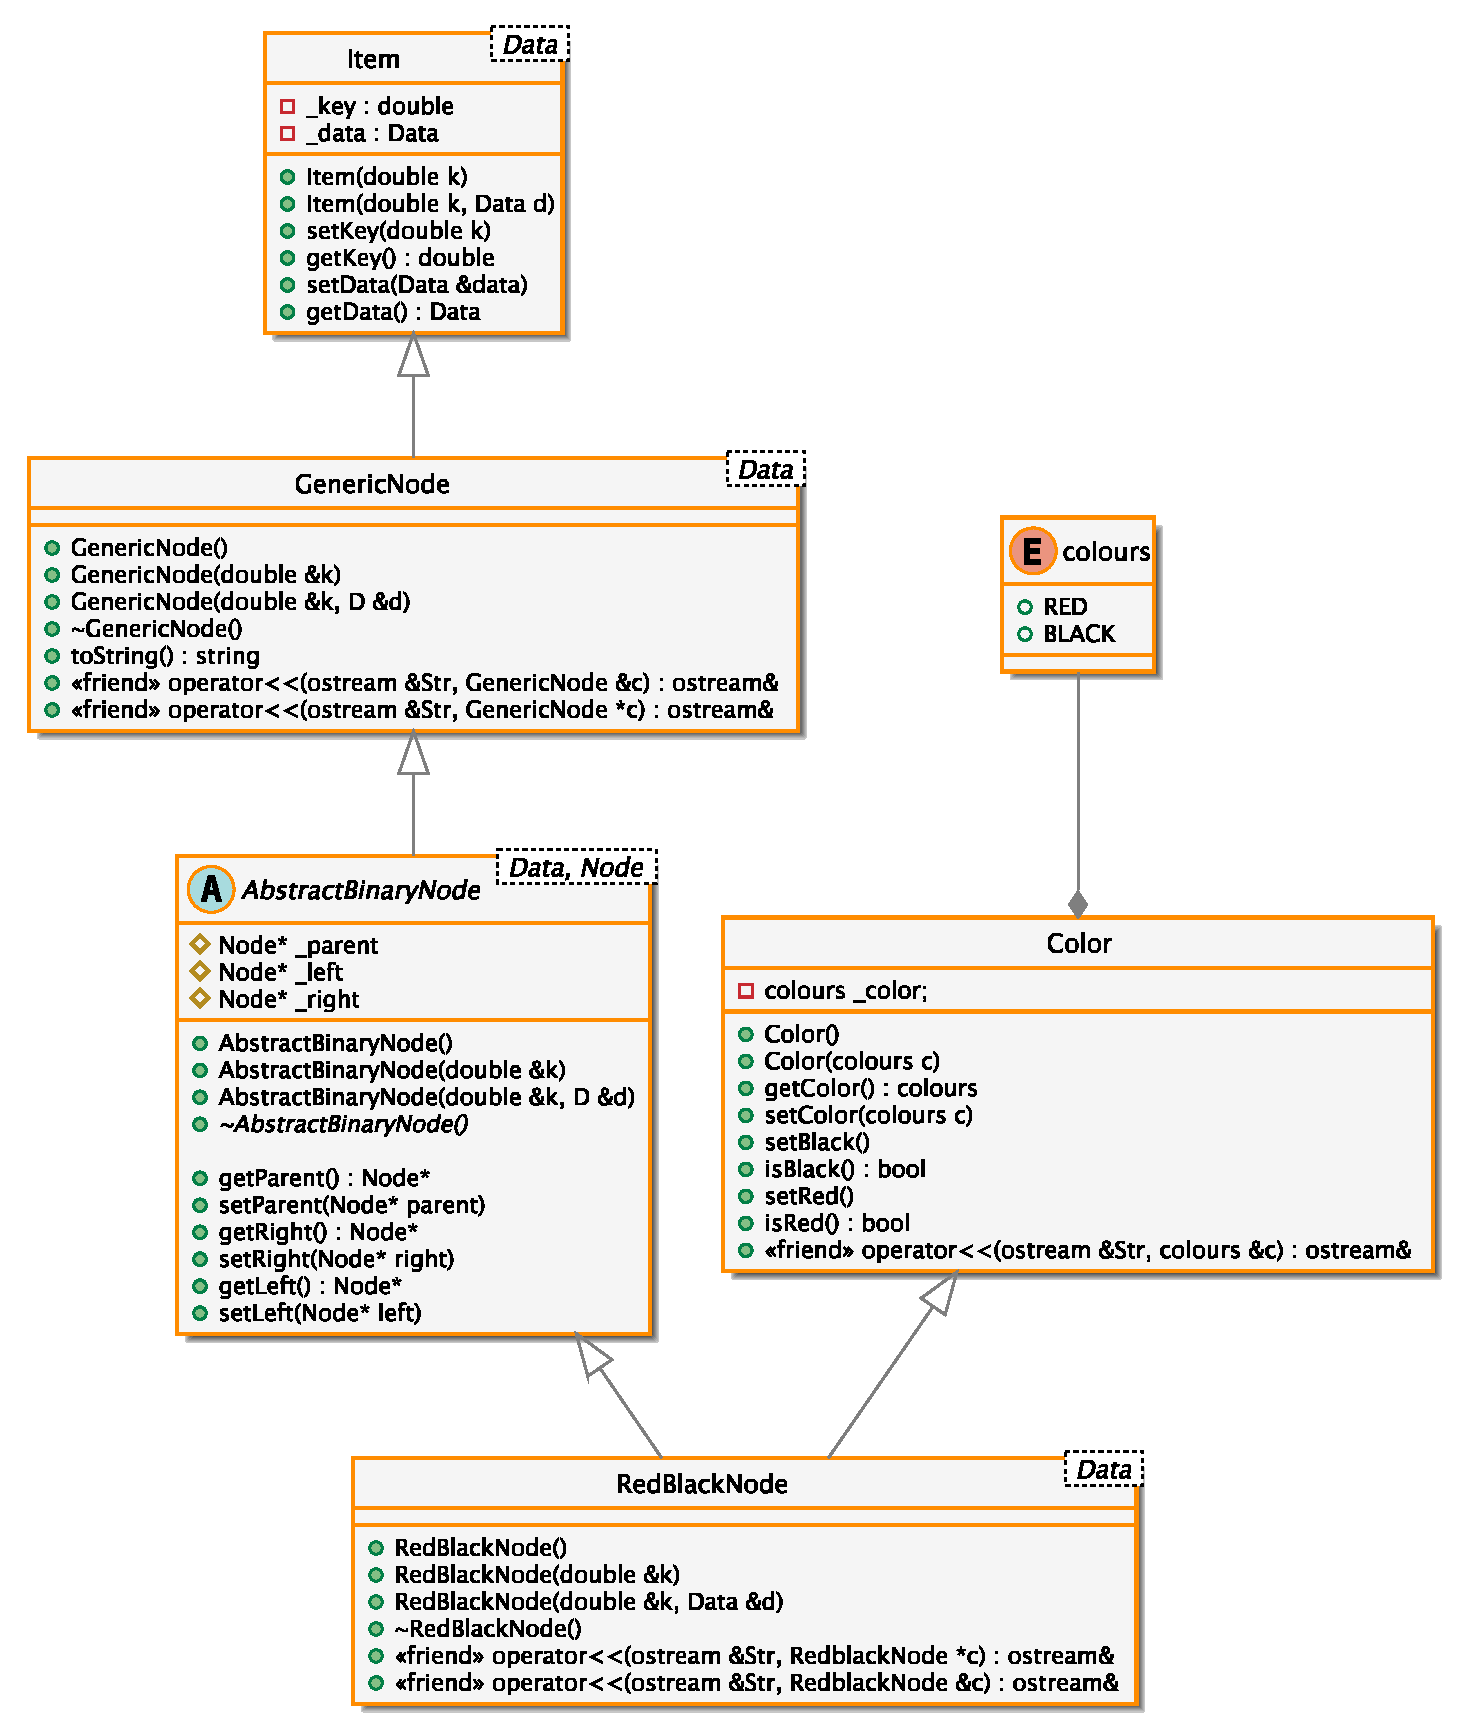
\includegraphics[scale=0.6]{tesina_tex/rbhash/2img/nodes.eps}
\captionof{figure}{Nodi degli alberi}
\end{center}
\subsubsection{Alberi}
Un albero Rosso Nero \`e un albero binario di ricerca auto
bilanciante, per tanto si \`e scelto di estendere la classe
BinarySearchTree ed aggiungere i metodi di supporto al bilanciamento. Inoltre due metodi virtuali (insert e delete), sono
stati ridefiniti nell'implementazione del Red Black.
\textit{insertNode} richiama tramite lo scope della classe
BinarySearchTree la insert e successivamente applica il
\textbf{fix} tipico dei red black.
\begin{center}
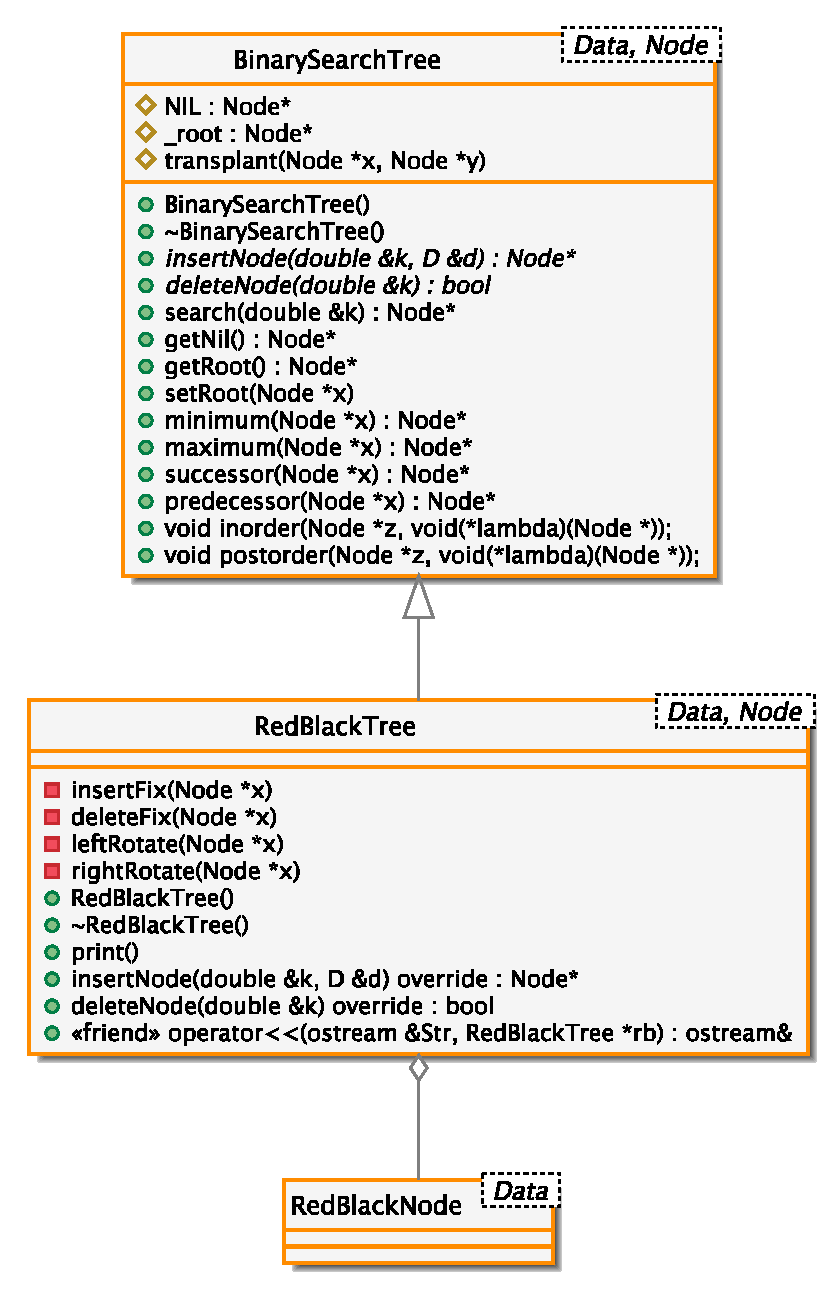
\includegraphics[scale=0.6]{tesina_tex/rbhash/2img/trees.eps}
\captionof{figure}{Alberi}
\end{center}
\subsection{Hash Table}
Onde evitare di dover riscrivere codice si \`e scelto di sfruttare
il nodo generico anche per l'\textbf{HashTable}. A tal proposito
si \`e sviluppato una tabella hash ad \textbf{indirizzamento aperto} che
prende in input come paramentro templato, il dato da conservare e 
la funzione di hash sotto forma di classe.
Per risolvere le collisioni si \`e scelto di usare due funzioni hash:
\texttt{k} \`e un valore double che indica
la chiave, $\texttt{i}$ \`e l'iteratore che al massimo 
$\texttt{m}$ volte \footnote{m \`e il size dell'hashtable}  
applicher\`a la funzione di hash. La prima restituisce un indice con valore compreso
tra $[0, m]$, mentre la seconda funzione di hash un valore compreso tra $[1, m-1]$. 
Verr\`a usata la prima funzione di hash e in caso di collisione
si riapplicher\`a
$h(i, m) = (h_1(k) + i * h_2(k)) \ mod \ m$. Sebbene con un costo 
computazionale pi\`u alto, il doppio hashing risolve le collisioni
pi\`u in fretta rispetto allispezione lineare o quadratica.\newline \indent 
La funzione $search()$ nella class \textbf{HashTable} usa due
diversi parametri di input per restituire valori diversi. Con la 
ricerca per valore si restituise, se disponibile un indice che 
usato nella seconda funzione di ricerca restituisce il dato.

\begin{center}
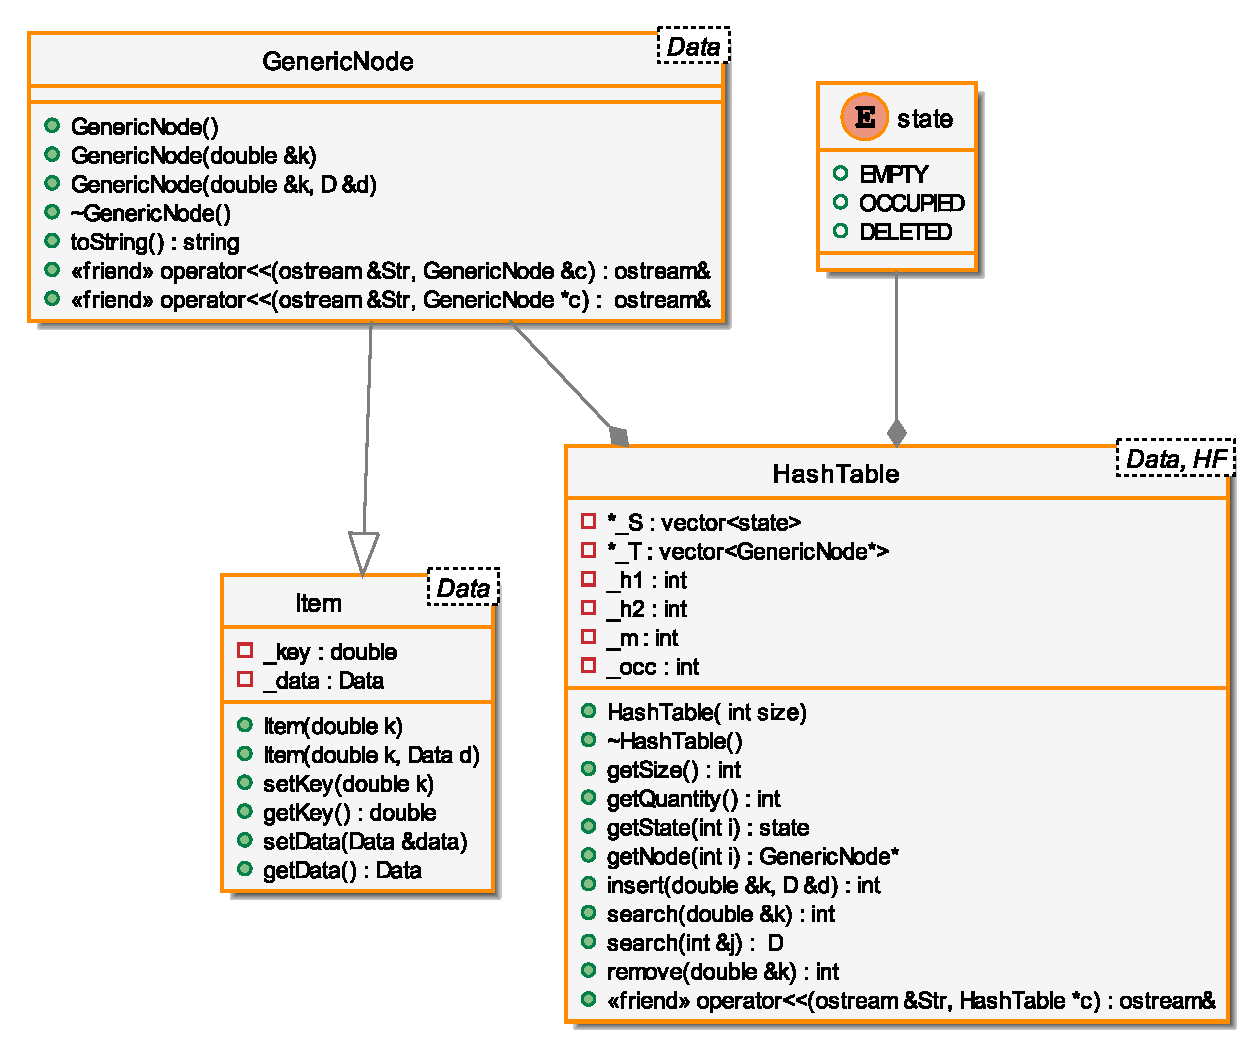
\includegraphics[scale=0.6]{tesina_tex/rbhash/2img/hash.eps}
\captionof{figure}{Hash Table}
\end{center}\newpage
\def\baselinestretch{1}
\section{Studio complessit\`a}
\def\baselinestretch{1.66}
\thispagestyle{headings}
La complessit\`a di tempo data dall'algoritmo galactic dijkstra \`e influenzata
dalle \textbf{due esecuzioni} (al pi\`u) del classico algoritmo di Dijkstra. Il calcolo
dei percorsi impiega $O(3E)$ poich\'e per raggiungere un nodo fino alla sorgente vuol dire
ripercorrere l'albero attraversando ogni arco nel caso peggiore, quindi mettendoci un tempo lineare.
Per cui si considerano le due applicazioni di Dijkstra che impiegano $O(2(V+E) 2log_2 V)$ che diventa
$O(2E2log_2 V)$ se ogni vertice \`e raggiungibile dalla sorgente, ma poich\`e è possibile portare
le costanti moltiplicative fuori diremo che la complessit\`a finale sar\`a $\mathbf{O(Elog_2V)}$.
L'algoritmo di Dijkstra impiega tale complessit\`a poich\'e influenzato dalle operazioni
$extractMin()$ e $decreaseKey()$ impiegate $|E|$ volte dalla coda di min priorit\`a basata
su min heap.
Si poteva pensare di usare un Heap di Fibonacci poich\'e si \`e notato che l'algoritmo
effettua pi\`u operazioni di $decreaseKey()$ che di $extractMin()$, e nella struttura dati
citata tale operazioni hanno rispettivamente costo computazionale $O(1)$ e $O(log_2V)$. Ci\`o
avrebbe comportato un miglioramento nel caso in cui ci fossero stati molti archi, avendo un costo
asintotico pari a $O(Vlog_2V +E)$.\newpage
\def\baselinestretch{1}
\section{Test e risultati}
\def\baselinestretch{1.66}
\thispagestyle{headings}

\subsection{Test effettuati}\label{notconn}
I risultati estratti da una shell dopo aver eseguito il programma prevedono vari grafi. Per ognuno
di essi vi sar\`a presente il grafico relativo.

\begin{center}
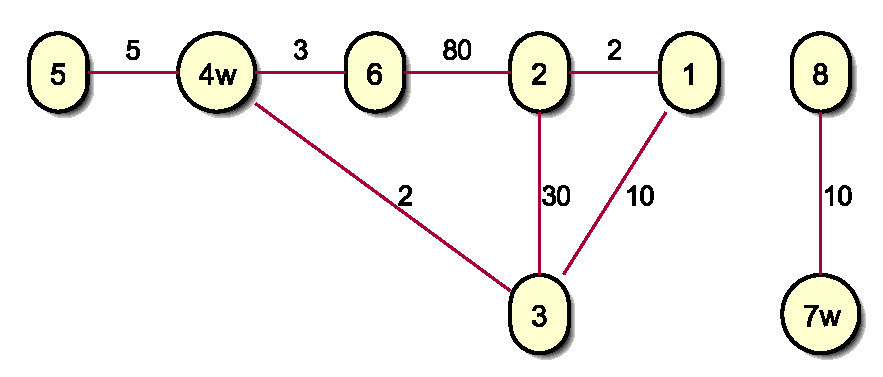
\includegraphics[scale=0.7]{tesina_tex/spacegraph/2img/notconn.eps}
\captionof{figure}{Grafo non connesso.}
\end{center}

\begin{minted}{bash}
Filling a graph with 8 nodes, 8 edges, 2 wormholes
STARTING READING FILE: 6
STARTING READING 2ndhalf: 2

Looking for a path from 1 to 8

Travel without wormholes: there are no paths that connect 1 with 8
        (disconnected graph)

Using wormholes -> [4, 7]: 1-3-4^7-8 in 23 unit time
\end{minted}

\newpage

\begin{center}
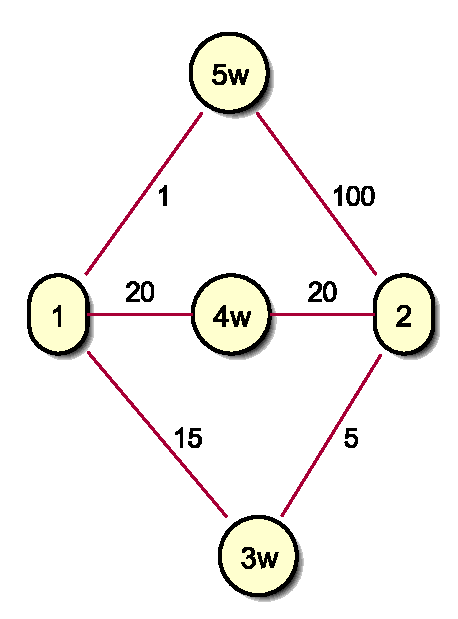
\includegraphics[scale=0.7]{tesina_tex/spacegraph/2img/diamond.eps}
\captionof{figure}{Grafo a diamante.}
\end{center}

\begin{minted}{bash}
Filling a graph with 5 nodes, 6 edges, 3 wormholes
STARTING READING FILE: 3
STARTING READING 2ndhalf: 3

Looking for a path from 1 to 2

Travel without wormholes: 1-3-2 in 20 time unit

Using wormholes -> [5, 3]: 1-5^3-2 in 7 unit time
\end{minted}



\newpage Nel grafo seguente il percorso con wormhole non \`e mostrato in quanto il wormhole
usato dalla sorgente e dalla destizione \`e lo stesso, infatti il nodo $11$ \`e presente
in entrambi i cammini minimi.
\begin{center}
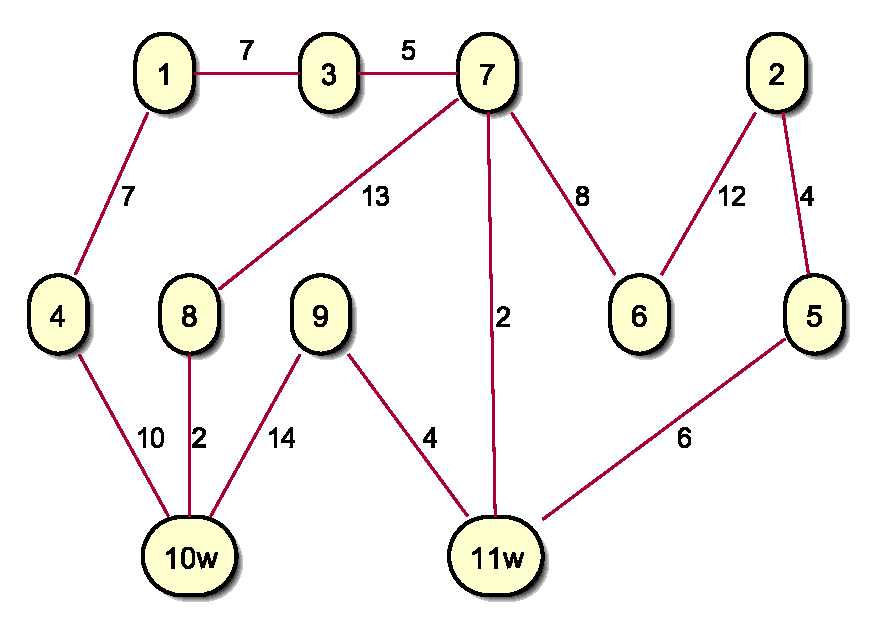
\includegraphics[scale=0.7]{tesina_tex/spacegraph/2img/traccia.eps}
\captionof{figure}{Grafo d'esempio.}
\end{center}

\begin{minted}{bash}
Filling a graph with 11 nodes, 13 edges, 2 wormholes
STARTING READING FILE: 11
STARTING READING 2ndhalf: 2

Looking for a path from 1 to 2

Travel without wormholes: 1-3-7-11-5-2 in 24 time unit

No fast travel with wormhole.
\end{minted}




\newpage Per puro stress testing del programma, si \`e utilizzato un file contentente
317080 nodi, 1049866 archi e 10 wormholes, ovviamente previo
commento nell'implementazione
del parser circa i controlli sull'input. Successimante si usa lo stesso file ma senza
wormhole in modo da non far applicare una seconda volta dijkstra.
Il risultato mostrato di seguito contiene l'esecuzione calcolandone i tempi tramite
l'applicativo \emph{time} presente nei sistemi operativi \emph{*NIX}

\begin{minted}[breaklines=true]{bash}
Filling a graph with 317080 nodes, 1049866 edges, 10 wormholes
STARTING READING FILE: 1049856
STARTING READING 2ndhalf: 10

Looking for a path from 316972 to 317029

Travel without wormholes:
316972-264079-298841-63506-59115-5530-26742-65338
-191800-287822-125483-121155-107180-308349-317029
in 104 time unit

Using wormholes -> [316972, 317029]: 316972^317029 in 1 unit time


real    1m42.700s
user    1m42.313s
sys     0m0.188s
\end{minted}
\newpage
Da notare come il file senza wormhole ci impiega circa la \textbf{met\`a}.

\begin{minted}[breaklines=true]{bash}
Filling a graph with 317080 nodes, 1049866 edges, 0 wormholes
STARTING READING FILE: 1049866
STARTING READING 2ndhalf: 0

Looking for a path from 316972 to 317029

Travel without wormholes:
316972-264079-298841-63506-59115-5530-26742-65338
-191800-287822-125483-121155-107180-308349-317029
in 104 time unit

No wormhole from Source to Destination.

real    0m56.303s
user    0m56.047s
sys     0m0.094s

\end{minted}

\newpage
\def\baselinestretch{1}
\section{Codice sorgente}
\def\baselinestretch{1.66}
\thispagestyle{headings}

\inputminted
[fontsize=\small,baselinestretch=1,
frame=lines,
framesep=10pt,
linenos=true,tabsize=2,
breaklines=true]{c++}{tesina_tex/source/graph/heap.hpp}
\inputminted
[fontsize=\small,baselinestretch=1,
frame=lines,
framesep=10pt,
linenos=true,tabsize=2,
breaklines=true]{c++}{tesina_tex/source/graph/heap.cpp}

\newpage
\inputminted
[fontsize=\small,baselinestretch=1,
frame=lines,
framesep=10pt,
linenos=true,tabsize=2,
breaklines=true]{c++}{tesina_tex/source/graph/minHeap.hpp}
\inputminted
[fontsize=\small,baselinestretch=1,
frame=lines,
framesep=10pt,
linenos=true,tabsize=2,
breaklines=true]{c++}{tesina_tex/source/graph/minHeap.cpp}
\newpage
\inputminted
[fontsize=\small,baselinestretch=1,
frame=lines,
framesep=10pt,
linenos=true,tabsize=2,
breaklines=true]{c++}{tesina_tex/source/graph/minPriorityQueue.hpp}
\inputminted
[fontsize=\small,baselinestretch=1,
frame=lines,
framesep=10pt,
linenos=true,tabsize=2,
breaklines=true]{c++}{tesina_tex/source/graph/minPriorityQueue.cpp}
\newpage


\inputminted
[fontsize=\small,baselinestretch=1,
frame=lines,
framesep=10pt,
linenos=true,tabsize=2,
breaklines=true]{c++}{tesina_tex/source/graph/galacticgraph.hpp}
\inputminted
[fontsize=\small,baselinestretch=1,
frame=lines,
framesep=10pt,
linenos=true,tabsize=2,
breaklines=true]{c++}{tesina_tex/source/graph/galacticgraph.cpp}
\newpage

\inputminted
[fontsize=\small,baselinestretch=1,
frame=lines,
framesep=10pt,
linenos=true,tabsize=2,
breaklines=true]{c++}{tesina_tex/source/graph/loader.hpp}
\inputminted
[fontsize=\small,baselinestretch=1,
frame=lines,
framesep=10pt,
linenos=true,tabsize=2,
breaklines=true]{c++}{tesina_tex/source/graph/loader.cpp}
\newpage

\inputminted
[fontsize=\small,baselinestretch=1,
frame=lines,
framesep=10pt,
linenos=true,tabsize=2,
breaklines=true]{c++}{tesina_tex/source/graph/debug.hpp}
\inputminted
[fontsize=\small,baselinestretch=1,
frame=lines,
framesep=10pt,
linenos=true,tabsize=2,
breaklines=true]{c++}{tesina_tex/source/graph/item.hpp}
\newpage

\inputminted
[fontsize=\small,baselinestretch=1,
frame=lines,
framesep=10pt,
linenos=true,tabsize=2,
breaklines=true]{c++}{tesina_tex/source/graph/vertex.hpp}
\inputminted
[fontsize=\small,baselinestretch=1,
frame=lines,
framesep=10pt,
linenos=true,tabsize=2,
breaklines=true]{c++}{tesina_tex/source/graph/vertex.cpp}
\newpage

\inputminted
[fontsize=\small,baselinestretch=1,
frame=lines,
framesep=10pt,
linenos=true,tabsize=2,
breaklines=true]{c++}{tesina_tex/source/graph/graph.hpp}
\inputminted
[fontsize=\small,baselinestretch=1,
frame=lines,
framesep=10pt,
linenos=true,tabsize=2,
breaklines=true]{c++}{tesina_tex/source/graph/graph.cpp}
\newpage\newpage
\newpage
\begin{thebibliography}{30}
    \bibitem{TOMCAT} Apache Tomcat \\
        \url{https://tomcat.apache.org/}
    \bibitem{H8} Hibernate middleware\\
        \url{https://hibernate.org/}
    \bibitem{WIKI} Wikipedia\\
        \url{https://wikipedia.org}
    \bibitem{BIGG} Google\\
        \url{https://www.google.com}
    \bibitem{SO} Stackoverflow\\
        \url{https://stackoverflow.com}
\end{thebibliography}
\newpage
    

\end{document}
